\section{Support Vector Machines}
Support vector machines are a set of supervised machine learning algorithms than can be used either for classification or regression proposed by Vapnik in 1963 \cite{VapLer63}. The main idea originates with binary classification and consists of finding an optimal hyper-plane between the data-points separating both target classes.

In its primal form, the support vector machine corresponds to the following minimization problem
\begin{equation}
    \begin{aligned}
& \underset{x}{\text{minimize}} 
& & \frac{1}{2}w^Tw + C \sum_{k=1}^N \xi_k \\
& \text{subject to}
& & y_i\left[ w \cdot x_i+b \right] \geq 1-\xi_i, \; i = 1, \ldots, N \\
& 
& & \xi_i \geq 0, \; i = 1, \ldots, N.
\end{aligned}
\end{equation}
We can now estimate a new data-point as
\begin{equation}
    \mathtt{SVM}(x) = w \cdot x + b 
\end{equation}
In comparison to other machine learning algorithms like neural networks for example, the SVMs present the big advantage taking the form of a convex optimization problem. But their greatest strength in my opinion is the ability to use transformations for representing a non-linear separation. Therefore, we have to to work in the dual space, where the SVM optimization problem now reformulates
\begin{equation}
    \begin{aligned}
& \underset{\alpha_i}{\text{maximize}} 
& & \sum_{i=1}^N \alpha_i - \frac12 \sum_{i,j=1}^N \alpha_i \alpha_j y_i y_j (x_i \cdot x_j) \\
& \text{subject to}
& & 0 \leq \alpha_i \leq C \; i = 1, \ldots, N \\
& 
& & \sum_{i=1}^N\alpha_i y_i = 0.
\end{aligned}
\end{equation}
and the estimation of a new data-point now becomes
\begin{equation}
    \mathtt{SVM}(x) = \sum_{i=1}^N \alpha_i y_i (x_i \cdot x) + b
\end{equation}
The feature vectors are only appearing in the form of a scalar product, which allows us to use Mercer's trick described in the previous section. Here again, we will use a \emph{radial based function} as kernel function ($K\left( x_i,x_j\right) = \exp\left(-\frac{\norm{x_i - x_j}^2}{2\sigma^2}\right)$). The SVM now becomes
\begin{equation}
    \begin{aligned}
& \underset{\alpha_i}{\text{maximize}} 
& & \sum_{i=1}^N \alpha_i - \frac12 \sum_{i,j=1}^N \alpha_i \alpha_j y_i y_j K(x_i, x_j) \\
& \text{subject to}
& & 0 \leq \alpha_i \leq C \; i = 1, \ldots, N \\
& 
& & \sum_{i=1}^N\alpha_i y_i = 0.
\end{aligned}
\end{equation}
with estimation
\begin{equation}
    \mathtt{SVM}(x) = \sum_{i=1}^N \alpha_i y_i K(x_i,x) + b
\end{equation}
However, there is also a downside: we are now facing an optimization problem in the dimension of the number of input instances and not of the dimension of the feature space anymore. This means that the number of support vector will drastically increase, which is a bad scenario for our privacy-friendly models. This is one of the investigated trade-offs.







\subsection{Multi-class SVMs}
The main problem of SVM for multi-class classification is that they are not natively suited for it. Indeed, SVM return a single number representing how far the tested data-point is from the hyperplane. SVMs are by definition created for binary classification as the whole idea behind it is to separate the feature space into two parts. The kernel trick doesn't change anything to that as it only projects the data-point into a space of higher --- often unlimited --- dimension where a new hyperplane is searched for, but still dividing this new higher dimension space into two parts.

Ideas for classifying SVMs into different classes could be for example to put the output number into bins. However, this is a very bad idea as it would in fact suggest that all the different classes are divided by parallel hyperplanes at a distances corresponding the the range of the bins, which range could also be trained (figure~\ref{mach:svm-model-gr-2}). It almost never occurs that one hyperplane separates two classes perfectly, the fact that $n-1$ parallel hyperplanes separate the feature space according the the $n$ different classes is even less likely. This hypothesis is much too strong and must be discarded. We therefore have to use more than one SVM and combine them.

We will present here two different ways of combining SVMs that have both been tested in the case of intrusion detection systems \cite{Kuang2014ADetection}\cite{SumaiyaThaseen2017IntrusionSVM} and produce fairly similar results although they never have been compared using exactly the same model for the rest.

The first way and the most frequent one is to create $n$ different classifiers, each for a class, and to look at which one produces the best results. 
\begin{equation}
    \underset{k}{\mathrm{arg}\,\mathrm{min}}\left\{ \mathtt{SVM}_k (x_i)   \right\}_{1 \ldots n} 
\end{equation}
where $\mathtt{SVM}_k$ represents the SVM for each class $k$. Each classifier takes as binary input, +1 for the class and -1 for all the rest data-points  (figure~\ref{mach:svm-model-1}). A way of interpreting it is looking for which SVM the data-point lies the farthest from the hyper-plane, at its good size (i.e. positive). This can be graphically observed at figure~\ref{mach:svm-model-gr-2}.

\begin{figure}[ht!]
    \centering
    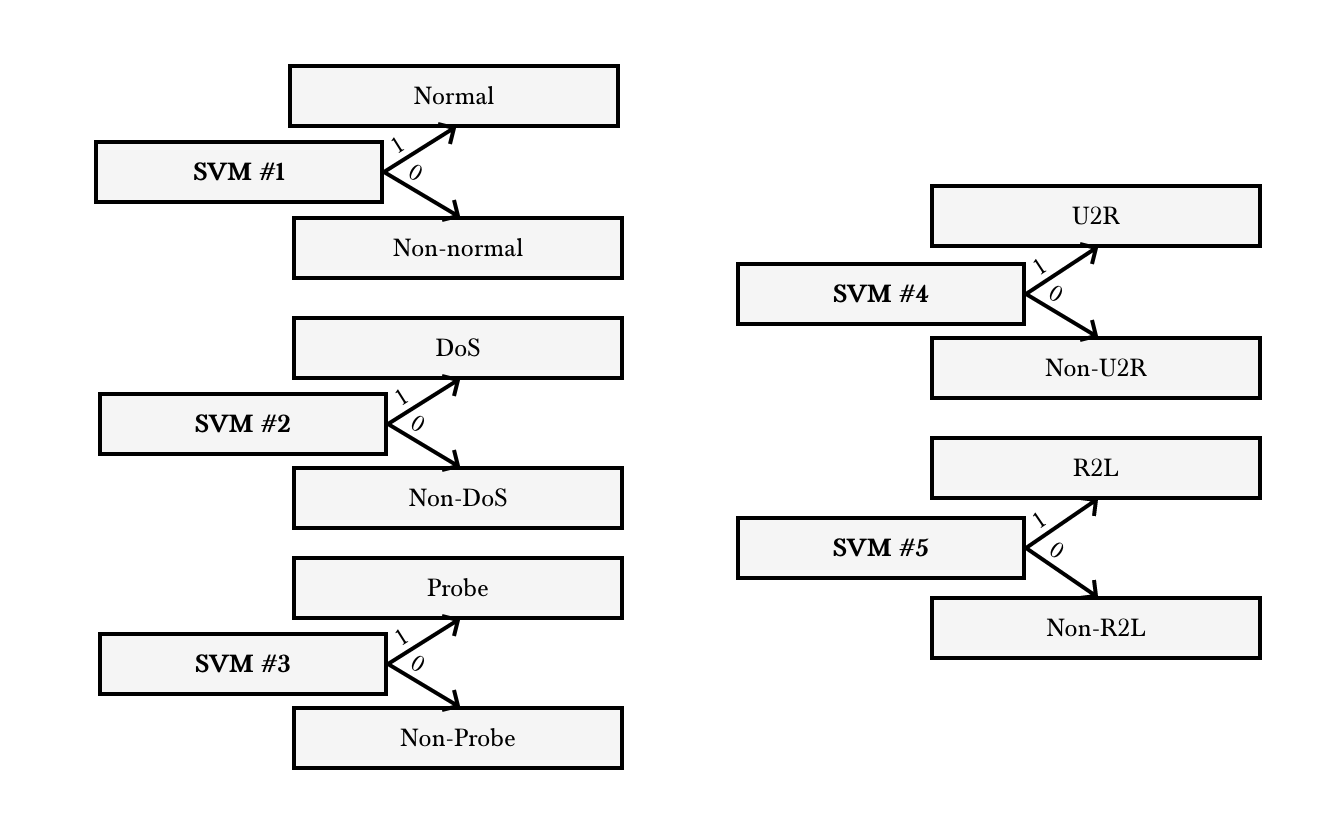
\includegraphics[width=.85\textwidth]{parts/chap-2/img-2/model-svm-1.png}
    \caption{Parallel multi-class SVM model.} 
    \label{mach:svm-model-1}
\end{figure}

Another way of doing it is to work with successive SVMs as in figure~\ref{mach:svm-model-2}. The first SVM is trained using one class as input versus all the others, as the first model. However the next classes are trained using one of the remaining classes versus the others remaining classes. The big advantage is that is only need $n-1$ different SVMs, which is one less compared to the previous model. Another advantage is that the last SVMs are trained one more specific data. However, the drawback is -- which is recurrent in series model --- that if one of the SVM isn't efficient, all the model is suffering. Graphically, this can be interpreted as first dividing the space with an hyper plane into two parts. One of the two parts is the subdivided into two new parts and so on (figure~\ref{mach:svm-model-gr-3}). Other tree structures are also to be considered, but this is not the scope of this thesis. We will limit ourselves to the consideration of these tree-structures in different orders. \noteH{(as they are the reason why we compare both is to compare the how reducing the number of support vector machines, in comparison to one-against-all models, may increase evaluation speed, not an internal study on the tree-based classifiers, which is a totally other subject. Limit myself to what I saw in papers and just add the answer to my wonder if the order has an influence.)}


\begin{figure}[ht!]
    \centering
    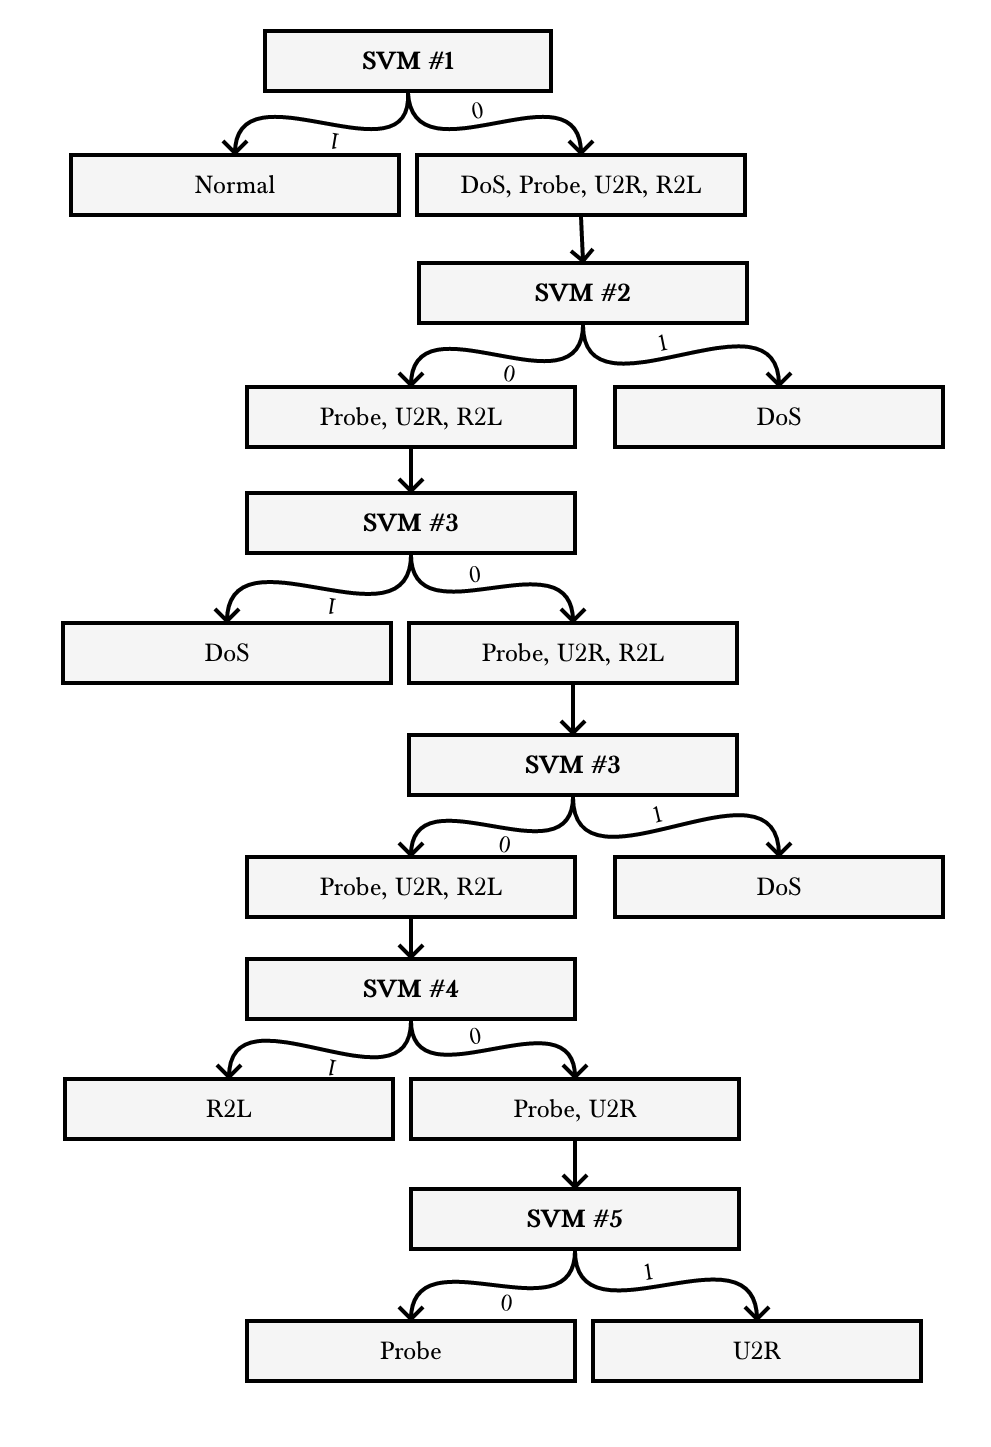
\includegraphics[width=.75\textwidth]{parts/chap-2/img-2/model-svm-2.png}
    \caption{Successive multi-class SVM model.} 
    \label{mach:svm-model-2}
\end{figure}

\begin{figure}
\begin{subfigure}[b]{0.32\textwidth}  
            \centering 
            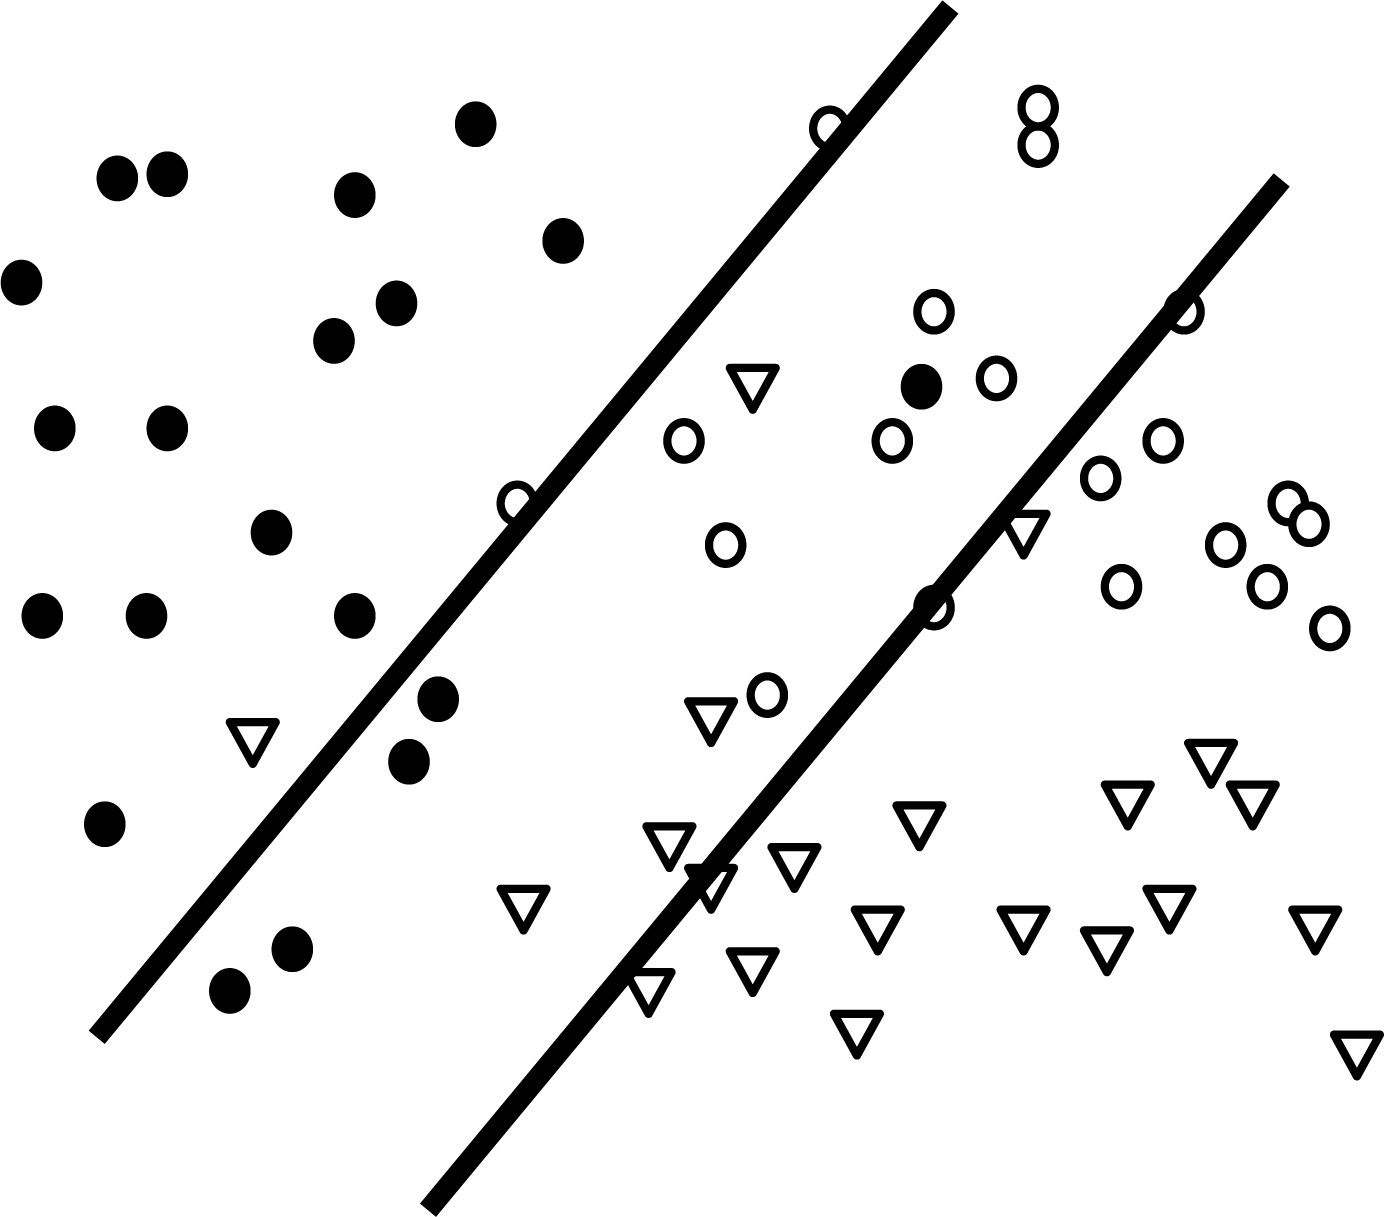
\includegraphics[width=.85\textwidth]{parts/chap-2/img-2/svm-par.png}
            \caption{Single SVM with bins.} 
            \label{mach:svm-model-gr-1}
        \end{subfigure}
        \hfill
        \begin{subfigure}[b]{0.32\textwidth}  
            \centering 
            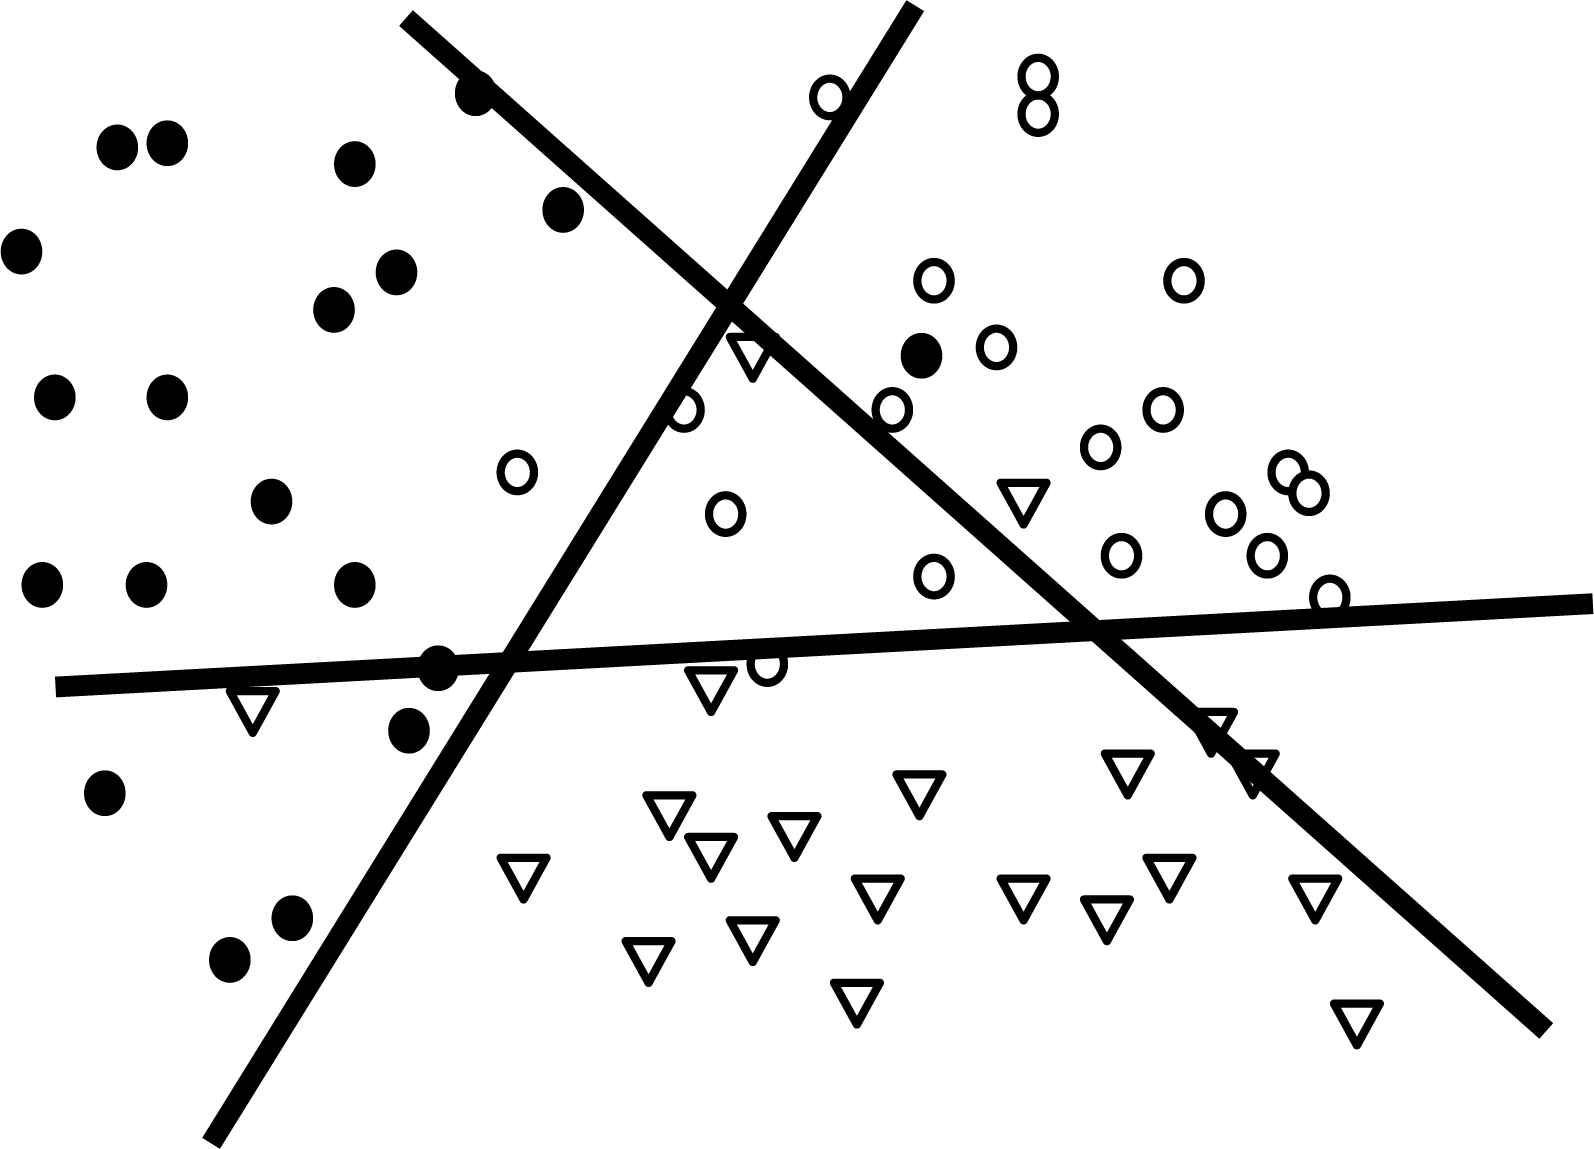
\includegraphics[width=.98\textwidth]{parts/chap-2/img-2/svm-multi.png}
            \caption{$n$ SVMs in parallel.} 
            \label{mach:svm-model-gr-2}
        \end{subfigure}
        \hfill
        \begin{subfigure}[b]{0.32\textwidth}   
            \centering 
            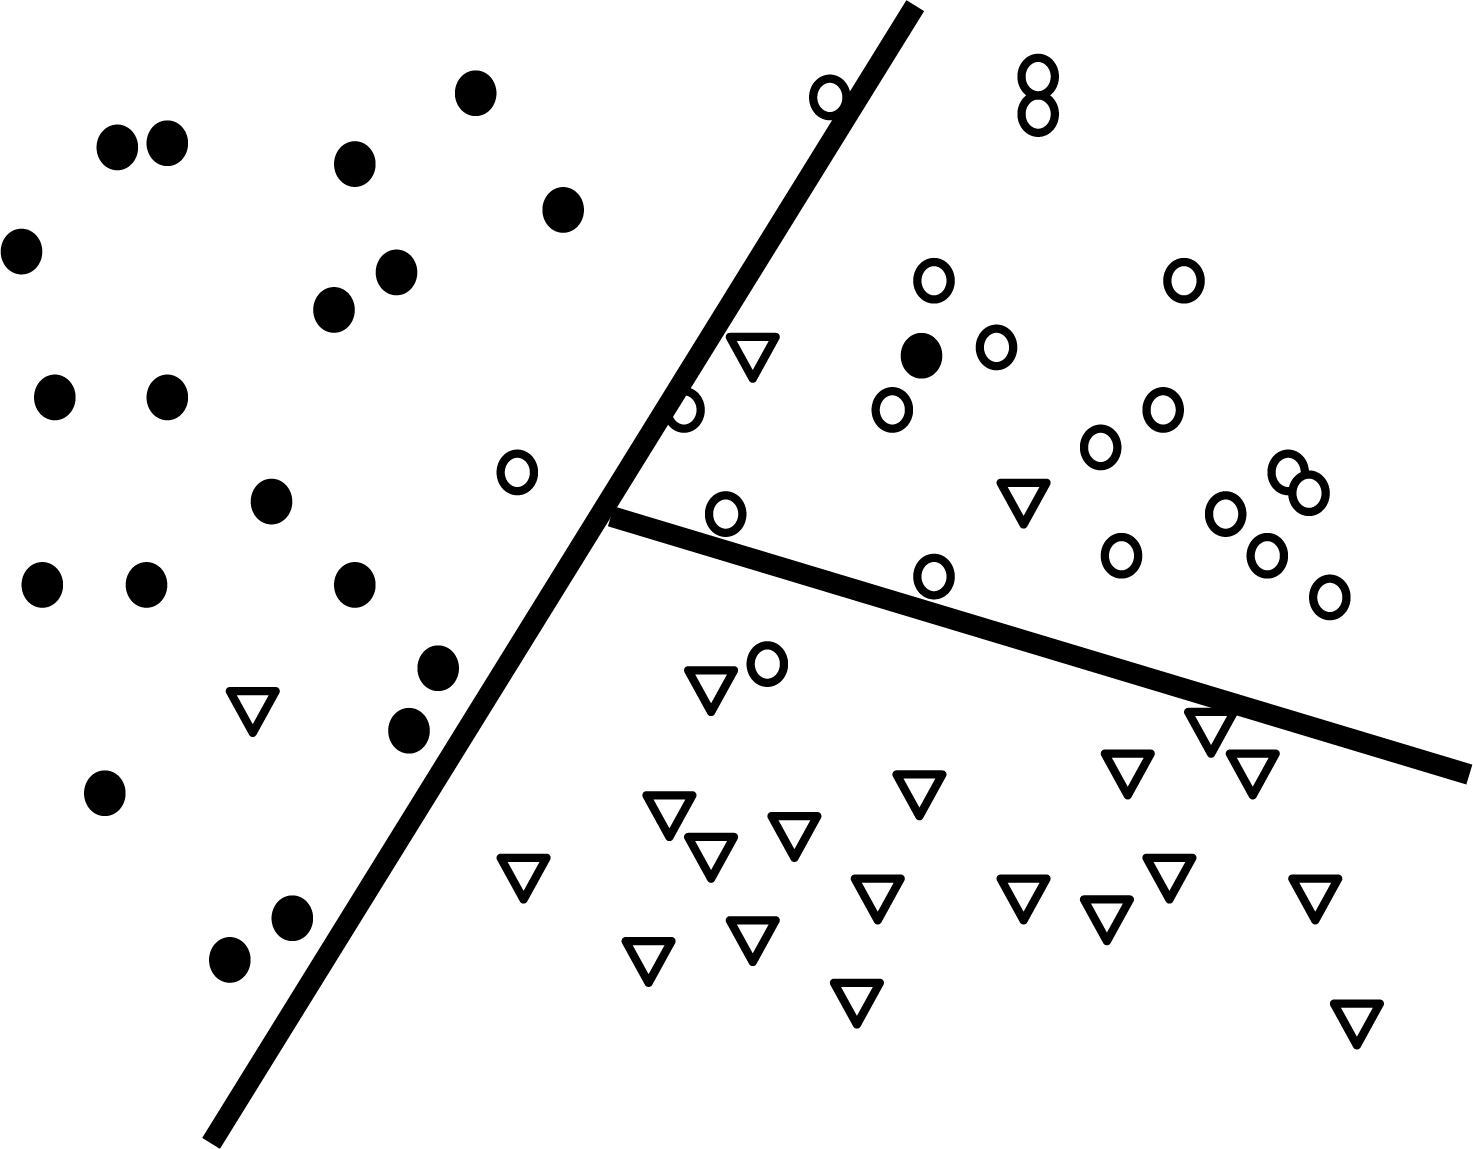
\includegraphics[width=.98\textwidth]{parts/chap-2/img-2/svm-seq.png}
            \caption{$n-1$ SVMs in sequence.} 
            \label{mach:svm-model-gr-3}
        \end{subfigure}
        \caption{Comparison of different multi-class models in the feature space. In this case, there are three classes $n=3$: dots, circles and triangles.}
\end{figure}


\FloatBarrier